\begin{frame}[fragile]{Visualização de update(2, 6, -3)}

    \begin{figure}
        \centering

        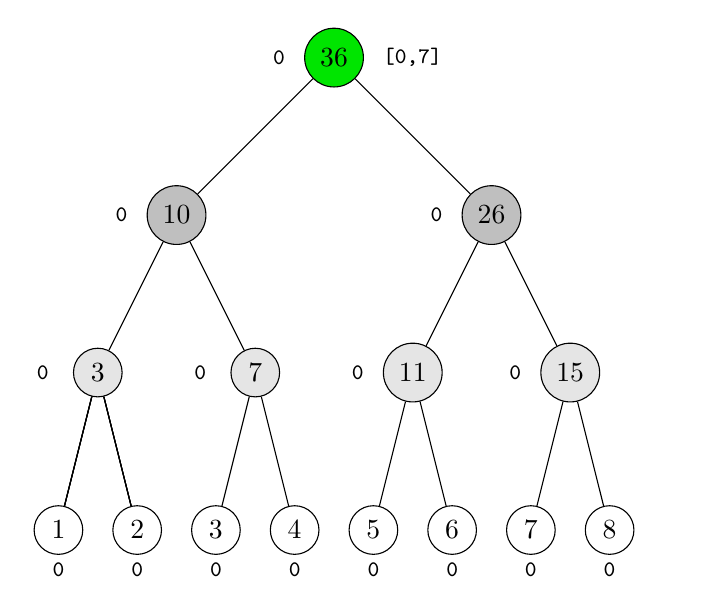
\begin{tikzpicture}
            \node[draw,circle] (A1) at (1, 0) { 1 };
            \node[draw,circle] (A2) at (2, 0) { 2 };
            \node[draw,circle] (A3) at (3, 0) { 3 };
            \node[draw,circle] (A4) at (4, 0) { 4 };
            \node[draw,circle] (A5) at (5, 0) { 5 };
            \node[draw,circle] (A6) at (6, 0) { 6 };
            \node[draw,circle] (A7) at (7, 0) { 7 };
            \node[draw,circle] (A8) at (8, 0) { 8 };

            \node at (1, -.5) { \footnotesize \texttt{\textbf{0}} };
            \node at (2, -.5) { \footnotesize \texttt{\textbf{0}} };
            \node at (3, -.5) { \footnotesize \texttt{\textbf{0}} };
            \node at (4, -.5) { \footnotesize \texttt{\textbf{0}} };
            \node at (5, -.5) { \footnotesize \texttt{\textbf{0}} };
            \node at (6, -.5) { \footnotesize \texttt{\textbf{0}} };
            \node at (7, -.5) { \footnotesize \texttt{\textbf{0}} };
            \node at (8, -.5) { \footnotesize \texttt{\textbf{0}} };
            \node[anchor=east] at (1, 2) { \footnotesize \texttt{\textbf{0}} };
            \node[anchor=east] at (3, 2) { \footnotesize \texttt{\textbf{0}} };
            \node[anchor=east] at (5, 2) { \footnotesize \texttt{\textbf{0}} };
            \node[anchor=east] at (7, 2) { \footnotesize \texttt{\textbf{0}} };
            \node[anchor=east] at (2, 4) { \footnotesize \texttt{\textbf{0}} };
            \node[anchor=east] at (6, 4) { \footnotesize \texttt{\textbf{0}} };
            \node[anchor=east] at (4, 6) { \footnotesize \texttt{\textbf{0}} };
            \node[anchor=west,opacity=0] at (8, 2) { \footnotesize \tt [6,7] };

            \node[draw,circle,fill=gray!20] (B1) at (1.5, 2) { 3 };
            \node[draw,circle,fill=gray!20] (B2) at (3.5, 2) { 7 };
            \node[draw,circle,fill=gray!20] (B3) at (5.5, 2) { 11 };
            \node[draw,circle,fill=gray!20] (B4) at (7.5, 2) { 15 };

            \node[draw,circle,fill=gray!50] (C1) at (2.5, 4) { 10 };
            \node[draw,circle,fill=gray!50] (C2) at (6.5, 4) { 26 };

            \node[draw,circle,fill=green!90!black] (D1) at (4.5, 6) { 36 };
            \node[anchor=west] at (5, 6) { \footnotesize \tt [0,7] };

            \draw (A1) -- (B1);
            \draw (A2) -- (B1);
            \draw (A3) -- (B2);
            \draw (A4) -- (B2);
            \draw (A5) -- (B3);
            \draw (A6) -- (B3);
            \draw (A7) -- (B4);
            \draw (A8) -- (B4);
            \draw (A1) -- (B1);
            \draw (A2) -- (B1);
            \draw (A1) -- (B1);
            \draw (A2) -- (B1);
            \draw (A1) -- (B1);
            \draw (A2) -- (B1);
            \draw (B1) -- (C1);
            \draw (B2) -- (C1);
            \draw (B3) -- (C2);
            \draw (B4) -- (C2);
            \draw (C1) -- (D1);
            \draw (C2) -- (D1);
        \end{tikzpicture}
    \end{figure}

\end{frame}

\begin{frame}[fragile]{Visualização de update(2, 6, -3)}

    \begin{figure}
        \centering

        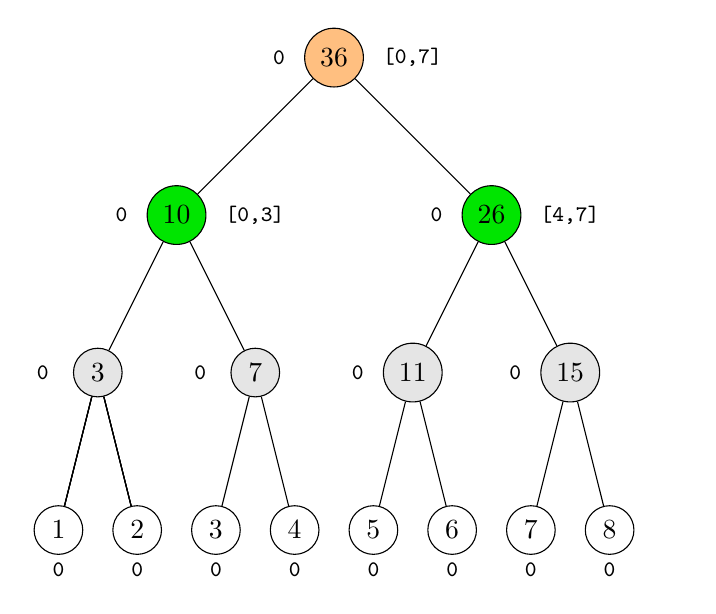
\begin{tikzpicture}
            \node[draw,circle] (A1) at (1, 0) { 1 };
            \node[draw,circle] (A2) at (2, 0) { 2 };
            \node[draw,circle] (A3) at (3, 0) { 3 };
            \node[draw,circle] (A4) at (4, 0) { 4 };
            \node[draw,circle] (A5) at (5, 0) { 5 };
            \node[draw,circle] (A6) at (6, 0) { 6 };
            \node[draw,circle] (A7) at (7, 0) { 7 };
            \node[draw,circle] (A8) at (8, 0) { 8 };

            \node at (1, -.5) { \footnotesize \texttt{\textbf{0}} };
            \node at (2, -.5) { \footnotesize \texttt{\textbf{0}} };
            \node at (3, -.5) { \footnotesize \texttt{\textbf{0}} };
            \node at (4, -.5) { \footnotesize \texttt{\textbf{0}} };
            \node at (5, -.5) { \footnotesize \texttt{\textbf{0}} };
            \node at (6, -.5) { \footnotesize \texttt{\textbf{0}} };
            \node at (7, -.5) { \footnotesize \texttt{\textbf{0}} };
            \node at (8, -.5) { \footnotesize \texttt{\textbf{0}} };
            \node[anchor=east] at (1, 2) { \footnotesize \texttt{\textbf{0}} };
            \node[anchor=east] at (3, 2) { \footnotesize \texttt{\textbf{0}} };
            \node[anchor=east] at (5, 2) { \footnotesize \texttt{\textbf{0}} };
            \node[anchor=east] at (7, 2) { \footnotesize \texttt{\textbf{0}} };
            \node[anchor=east] at (2, 4) { \footnotesize \texttt{\textbf{0}} };
            \node[anchor=east] at (6, 4) { \footnotesize \texttt{\textbf{0}} };
            \node[anchor=east] at (4, 6) { \footnotesize \texttt{\textbf{0}} };
            \node[anchor=west,opacity=0] at (8, 2) { \footnotesize \tt [6,7] };

            \node[draw,circle,fill=gray!20] (B1) at (1.5, 2) { 3 };
            \node[draw,circle,fill=gray!20] (B2) at (3.5, 2) { 7 };
            \node[draw,circle,fill=gray!20] (B3) at (5.5, 2) { 11 };
            \node[draw,circle,fill=gray!20] (B4) at (7.5, 2) { 15 };
            \node[anchor=west,opacity=0] at (8, 2) { \footnotesize \tt [6,7] };

            \node[draw,circle,fill=green!90!black] (C1) at (2.5, 4) { 10 };
            \node[anchor=west] at (3, 4) { \footnotesize \tt [0,3] };

            \node[draw,circle,fill=green!90!black] (C2) at (6.5, 4) { 26 };
            \node[anchor=west] at (7, 4) { \footnotesize \tt [4,7] };

            \node[draw,circle,fill=orange!50] (D1) at (4.5, 6) { 36 };
            \node[anchor=west] at (5, 6) { \footnotesize \tt [0,7] };

            \draw (A1) -- (B1);
            \draw (A2) -- (B1);
            \draw (A3) -- (B2);
            \draw (A4) -- (B2);
            \draw (A5) -- (B3);
            \draw (A6) -- (B3);
            \draw (A7) -- (B4);
            \draw (A8) -- (B4);
            \draw (A1) -- (B1);
            \draw (A2) -- (B1);
            \draw (A1) -- (B1);
            \draw (A2) -- (B1);
            \draw (A1) -- (B1);
            \draw (A2) -- (B1);
            \draw (B1) -- (C1);
            \draw (B2) -- (C1);
            \draw (B3) -- (C2);
            \draw (B4) -- (C2);
            \draw (C1) -- (D1);
            \draw (C2) -- (D1);
        \end{tikzpicture}
    \end{figure}

\end{frame}

\begin{frame}[fragile]{Visualização de update(2, 6, -3)}

    \begin{figure}
        \centering

        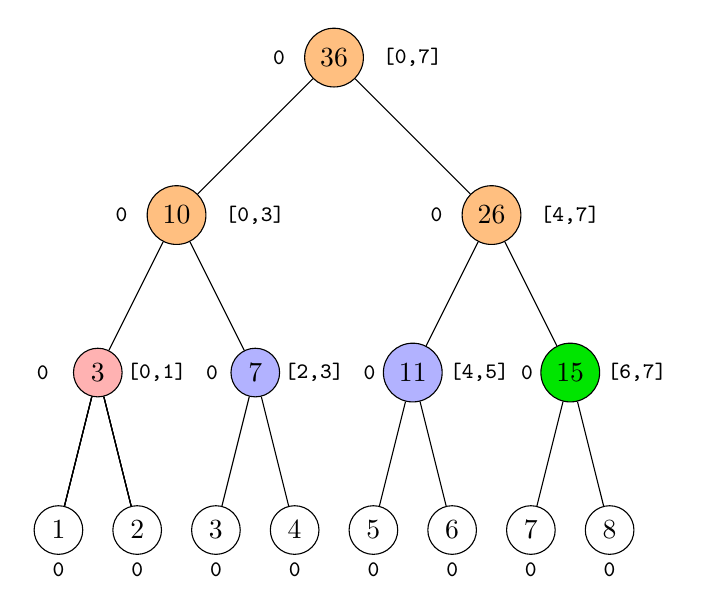
\begin{tikzpicture}
            \node[draw,circle] (A1) at (1, 0) { 1 };
            \node[draw,circle] (A2) at (2, 0) { 2 };
            \node[draw,circle] (A3) at (3, 0) { 3 };
            \node[draw,circle] (A4) at (4, 0) { 4 };
            \node[draw,circle] (A5) at (5, 0) { 5 };
            \node[draw,circle] (A6) at (6, 0) { 6 };
            \node[draw,circle] (A7) at (7, 0) { 7 };
            \node[draw,circle] (A8) at (8, 0) { 8 };

            \node at (1, -.5) { \footnotesize \texttt{\textbf{0}} };
            \node at (2, -.5) { \footnotesize \texttt{\textbf{0}} };
            \node at (3, -.5) { \footnotesize \texttt{\textbf{0}} };
            \node at (4, -.5) { \footnotesize \texttt{\textbf{0}} };
            \node at (5, -.5) { \footnotesize \texttt{\textbf{0}} };
            \node at (6, -.5) { \footnotesize \texttt{\textbf{0}} };
            \node at (7, -.5) { \footnotesize \texttt{\textbf{0}} };
            \node at (8, -.5) { \footnotesize \texttt{\textbf{0}} };
            \node[anchor=east] at (1, 2) { \footnotesize \texttt{\textbf{0}} };
            \node[anchor=east] at (3.15, 2) { \footnotesize \texttt{\textbf{0}} };
            \node[anchor=east] at (5.15, 2) { \footnotesize \texttt{\textbf{0}} };
            \node[anchor=east] at (7.15, 2) { \footnotesize \texttt{\textbf{0}} };
            \node[anchor=east] at (2, 4) { \footnotesize \texttt{\textbf{0}} };
            \node[anchor=east] at (6, 4) { \footnotesize \texttt{\textbf{0}} };
            \node[anchor=east] at (4, 6) { \footnotesize \texttt{\textbf{0}} };
            \node[anchor=west,opacity=0] at (8, 2) { \footnotesize \tt [6,7] };

            \node[draw,circle,fill=red!30] (B1) at (1.5, 2) { 3 };
            \node[anchor=west] at (1.75, 2) { \footnotesize \tt [0,1] };

            \node[draw,circle,fill=blue!30] (B2) at (3.5, 2) { 7 };
            \node[anchor=west] at (3.75, 2) { \footnotesize \tt [2,3] };

            \node[draw,circle,fill=blue!30] (B3) at (5.5, 2) { 11 };
            \node[anchor=west] at (5.85, 2) { \footnotesize \tt [4,5] };

            \node[draw,circle,fill=green!90!black] (B4) at (7.5, 2) { 15 };
            \node[anchor=west] at (7.85, 2) { \footnotesize \tt [6,7] };

            \node[draw,circle,fill=orange!50] (C1) at (2.5, 4) { 10 };
            \node[anchor=west] at (3, 4) { \footnotesize \tt [0,3] };

            \node[draw,circle,fill=orange!50] (C2) at (6.5, 4) { 26 };
            \node[anchor=west] at (7, 4) { \footnotesize \tt [4,7] };

            \node[draw,circle,fill=orange!50] (D1) at (4.5, 6) { 36 };
            \node[anchor=west] at (5, 6) { \footnotesize \tt [0,7] };

            \draw (A1) -- (B1);
            \draw (A2) -- (B1);
            \draw (A3) -- (B2);
            \draw (A4) -- (B2);
            \draw (A5) -- (B3);
            \draw (A6) -- (B3);
            \draw (A7) -- (B4);
            \draw (A8) -- (B4);
            \draw (A1) -- (B1);
            \draw (A2) -- (B1);
            \draw (A1) -- (B1);
            \draw (A2) -- (B1);
            \draw (A1) -- (B1);
            \draw (A2) -- (B1);
            \draw (B1) -- (C1);
            \draw (B2) -- (C1);
            \draw (B3) -- (C2);
            \draw (B4) -- (C2);
            \draw (C1) -- (D1);
            \draw (C2) -- (D1);
        \end{tikzpicture}
    \end{figure}

\end{frame}

\begin{frame}[fragile]{Visualização de update(2, 6, -3)}

    \begin{figure}
        \centering

        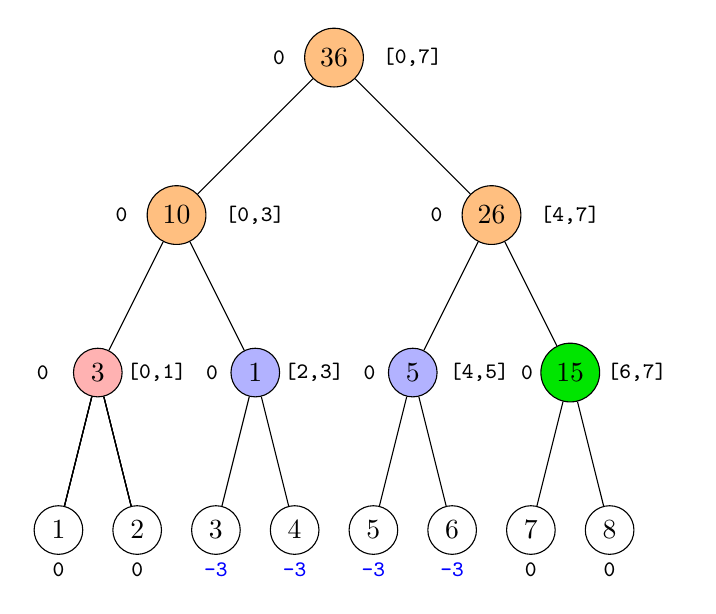
\begin{tikzpicture}
            \node[draw,circle] (A1) at (1, 0) { 1 };
            \node[draw,circle] (A2) at (2, 0) { 2 };
            \node[draw,circle] (A3) at (3, 0) { 3 };
            \node[draw,circle] (A4) at (4, 0) { 4 };
            \node[draw,circle] (A5) at (5, 0) { 5 };
            \node[draw,circle] (A6) at (6, 0) { 6 };
            \node[draw,circle] (A7) at (7, 0) { 7 };
            \node[draw,circle] (A8) at (8, 0) { 8 };

            \node at (1, -.5) { \footnotesize \texttt{\textbf{0}} };
            \node at (2, -.5) { \footnotesize \texttt{\textbf{0}} };
            \node at (3, -.5) { \footnotesize \textcolor{blue}{\texttt{\textbf{-3}}} };
            \node at (4, -.5) { \footnotesize \textcolor{blue}{\texttt{\textbf{-3}}} };
            \node at (5, -.5) { \footnotesize \textcolor{blue}{\texttt{\textbf{-3}}} };
            \node at (6, -.5) { \footnotesize \textcolor{blue}{\texttt{\textbf{-3}}} };
            \node at (7, -.5) { \footnotesize \texttt{\textbf{0}} };
            \node at (8, -.5) { \footnotesize \texttt{\textbf{0}} };
            \node[anchor=east] at (1, 2) { \footnotesize \texttt{\textbf{0}} };
            \node[anchor=east] at (3.15, 2) { \footnotesize \texttt{\textbf{0}} };
            \node[anchor=east] at (5.15, 2) { \footnotesize \texttt{\textbf{0}} };
            \node[anchor=east] at (7.15, 2) { \footnotesize \texttt{\textbf{0}} };
            \node[anchor=east] at (2, 4) { \footnotesize \texttt{\textbf{0}} };
            \node[anchor=east] at (6, 4) { \footnotesize \texttt{\textbf{0}} };
            \node[anchor=east] at (4, 6) { \footnotesize \texttt{\textbf{0}} };
            \node[anchor=west,opacity=0] at (8, 2) { \footnotesize \tt [6,7] };

            \node[draw,circle,fill=red!30] (B1) at (1.5, 2) { 3 };
            \node[anchor=west] at (1.75, 2) { \footnotesize \tt [0,1] };

            \node[draw,circle,fill=blue!30] (B2) at (3.5, 2) { 1 };
            \node[anchor=west] at (3.75, 2) { \footnotesize \tt [2,3] };

            \node[draw,circle,fill=blue!30] (B3) at (5.5, 2) { 5 };
            \node[anchor=west] at (5.85, 2) { \footnotesize \tt [4,5] };

            \node[draw,circle,fill=green!90!black] (B4) at (7.5, 2) { 15 };
            \node[anchor=west] at (7.85, 2) { \footnotesize \tt [6,7] };

            \node[draw,circle,fill=orange!50] (C1) at (2.5, 4) { 10 };
            \node[anchor=west] at (3, 4) { \footnotesize \tt [0,3] };

            \node[draw,circle,fill=orange!50] (C2) at (6.5, 4) { 26 };
            \node[anchor=west] at (7, 4) { \footnotesize \tt [4,7] };

            \node[draw,circle,fill=orange!50] (D1) at (4.5, 6) { 36 };
            \node[anchor=west] at (5, 6) { \footnotesize \tt [0,7] };

            \draw (A1) -- (B1);
            \draw (A2) -- (B1);
            \draw (A3) -- (B2);
            \draw (A4) -- (B2);
            \draw (A5) -- (B3);
            \draw (A6) -- (B3);
            \draw (A7) -- (B4);
            \draw (A8) -- (B4);
            \draw (A1) -- (B1);
            \draw (A2) -- (B1);
            \draw (A1) -- (B1);
            \draw (A2) -- (B1);
            \draw (A1) -- (B1);
            \draw (A2) -- (B1);
            \draw (B1) -- (C1);
            \draw (B2) -- (C1);
            \draw (B3) -- (C2);
            \draw (B4) -- (C2);
            \draw (C1) -- (D1);
            \draw (C2) -- (D1);
        \end{tikzpicture}
    \end{figure}

\end{frame}

\begin{frame}[fragile]{Visualização de update(2, 6, -3)}

    \begin{figure}
        \centering

        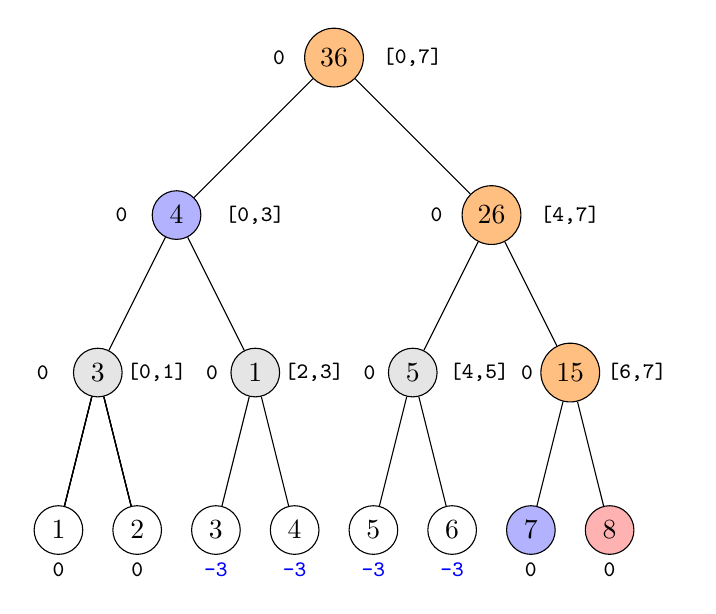
\begin{tikzpicture}
            \node[draw,circle] (A1) at (1, 0) { 1 };
            \node[draw,circle] (A2) at (2, 0) { 2 };
            \node[draw,circle] (A3) at (3, 0) { 3 };
            \node[draw,circle] (A4) at (4, 0) { 4 };
            \node[draw,circle] (A5) at (5, 0) { 5 };
            \node[draw,circle] (A6) at (6, 0) { 6 };
            \node[draw,circle,fill=blue!30] (A7) at (7, 0) { 7 };
            \node[draw,circle,fill=red!30] (A8) at (8, 0) { 8 };

            \node at (1, -.5) { \footnotesize \texttt{\textbf{0}} };
            \node at (2, -.5) { \footnotesize \texttt{\textbf{0}} };
            \node at (3, -.5) { \footnotesize \textcolor{blue}{\texttt{\textbf{-3}}} };
            \node at (4, -.5) { \footnotesize \textcolor{blue}{\texttt{\textbf{-3}}} };
            \node at (5, -.5) { \footnotesize \textcolor{blue}{\texttt{\textbf{-3}}} };
            \node at (6, -.5) { \footnotesize \textcolor{blue}{\texttt{\textbf{-3}}} };
            \node at (7, -.5) { \footnotesize \texttt{\textbf{0}} };
            \node at (8, -.5) { \footnotesize \texttt{\textbf{0}} };
            \node[anchor=east] at (1, 2) { \footnotesize \texttt{\textbf{0}} };
            \node[anchor=east] at (3.15, 2) { \footnotesize \texttt{\textbf{0}} };
            \node[anchor=east] at (5.15, 2) { \footnotesize \texttt{\textbf{0}} };
            \node[anchor=east] at (7.15, 2) { \footnotesize \texttt{\textbf{0}} };
            \node[anchor=east] at (2, 4) { \footnotesize \texttt{\textbf{0}} };
            \node[anchor=east] at (6, 4) { \footnotesize \texttt{\textbf{0}} };
            \node[anchor=east] at (4, 6) { \footnotesize \texttt{\textbf{0}} };
            \node[anchor=west,opacity=0] at (8, 2) { \footnotesize \tt [6,7] };

            \node[draw,circle,fill=gray!20] (B1) at (1.5, 2) { 3 };
            \node[anchor=west] at (1.75, 2) { \footnotesize \tt [0,1] };

            \node[draw,circle,fill=gray!20] (B2) at (3.5, 2) { 1 };
            \node[anchor=west] at (3.75, 2) { \footnotesize \tt [2,3] };

            \node[draw,circle,fill=gray!20] (B3) at (5.5, 2) { 5 };
            \node[anchor=west] at (5.85, 2) { \footnotesize \tt [4,5] };

            \node[draw,circle,fill=orange!50] (B4) at (7.5, 2) { 15 };
            \node[anchor=west] at (7.85, 2) { \footnotesize \tt [6,7] };

            \node[draw,circle,fill=blue!30] (C1) at (2.5, 4) { 4 };
            \node[anchor=west] at (3, 4) { \footnotesize \tt [0,3] };

            \node[draw,circle,fill=orange!50] (C2) at (6.5, 4) { 26 };
            \node[anchor=west] at (7, 4) { \footnotesize \tt [4,7] };

            \node[draw,circle,fill=orange!50] (D1) at (4.5, 6) { 36 };
            \node[anchor=west] at (5, 6) { \footnotesize \tt [0,7] };

            \draw (A1) -- (B1);
            \draw (A2) -- (B1);
            \draw (A3) -- (B2);
            \draw (A4) -- (B2);
            \draw (A5) -- (B3);
            \draw (A6) -- (B3);
            \draw (A7) -- (B4);
            \draw (A8) -- (B4);
            \draw (A1) -- (B1);
            \draw (A2) -- (B1);
            \draw (A1) -- (B1);
            \draw (A2) -- (B1);
            \draw (A1) -- (B1);
            \draw (A2) -- (B1);
            \draw (B1) -- (C1);
            \draw (B2) -- (C1);
            \draw (B3) -- (C2);
            \draw (B4) -- (C2);
            \draw (C1) -- (D1);
            \draw (C2) -- (D1);
        \end{tikzpicture}
    \end{figure}

\end{frame}

\begin{frame}[fragile]{Visualização de update(2, 6, -3)}

    \begin{figure}
        \centering

        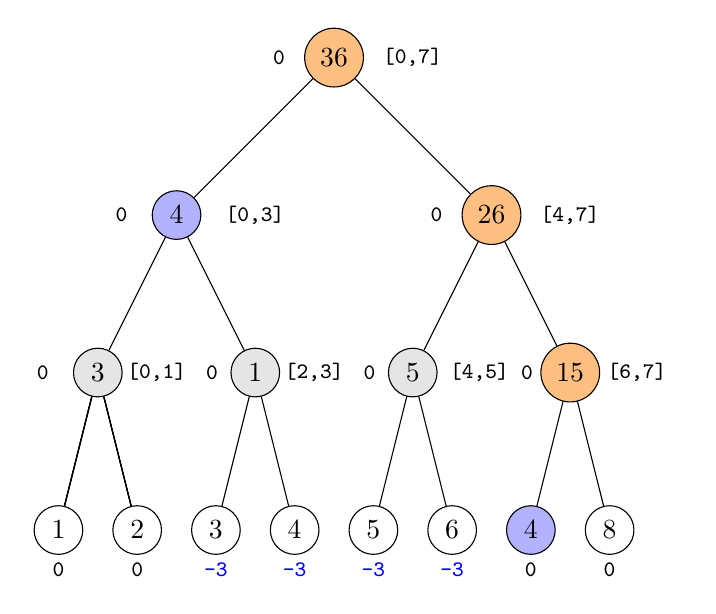
\begin{tikzpicture}
            \node[draw,circle] (A1) at (1, 0) { 1 };
            \node[draw,circle] (A2) at (2, 0) { 2 };
            \node[draw,circle] (A3) at (3, 0) { 3 };
            \node[draw,circle] (A4) at (4, 0) { 4 };
            \node[draw,circle] (A5) at (5, 0) { 5 };
            \node[draw,circle] (A6) at (6, 0) { 6 };
            \node[draw,circle,fill=blue!30] (A7) at (7, 0) { 4 };
            \node[draw,circle] (A8) at (8, 0) { 8 };

            \node at (1, -.5) { \footnotesize \texttt{\textbf{0}} };
            \node at (2, -.5) { \footnotesize \texttt{\textbf{0}} };
            \node at (3, -.5) { \footnotesize \textcolor{blue}{\texttt{\textbf{-3}}} };
            \node at (4, -.5) { \footnotesize \textcolor{blue}{\texttt{\textbf{-3}}} };
            \node at (5, -.5) { \footnotesize \textcolor{blue}{\texttt{\textbf{-3}}} };
            \node at (6, -.5) { \footnotesize \textcolor{blue}{\texttt{\textbf{-3}}} };
            \node at (7, -.5) { \footnotesize \texttt{\textbf{0}} };
            \node at (8, -.5) { \footnotesize \texttt{\textbf{0}} };
            \node[anchor=east] at (1, 2) { \footnotesize \texttt{\textbf{0}} };
            \node[anchor=east] at (3.15, 2) { \footnotesize \texttt{\textbf{0}} };
            \node[anchor=east] at (5.15, 2) { \footnotesize \texttt{\textbf{0}} };
            \node[anchor=east] at (7.15, 2) { \footnotesize \texttt{\textbf{0}} };
            \node[anchor=east] at (2, 4) { \footnotesize \texttt{\textbf{0}} };
            \node[anchor=east] at (6, 4) { \footnotesize \texttt{\textbf{0}} };
            \node[anchor=east] at (4, 6) { \footnotesize \texttt{\textbf{0}} };
            \node[anchor=west,opacity=0] at (8, 2) { \footnotesize \tt [6,7] };

            \node[draw,circle,fill=gray!20] (B1) at (1.5, 2) { 3 };
            \node[anchor=west] at (1.75, 2) { \footnotesize \tt [0,1] };

            \node[draw,circle,fill=gray!20] (B2) at (3.5, 2) { 1 };
            \node[anchor=west] at (3.75, 2) { \footnotesize \tt [2,3] };

            \node[draw,circle,fill=gray!20] (B3) at (5.5, 2) { 5 };
            \node[anchor=west] at (5.85, 2) { \footnotesize \tt [4,5] };

            \node[draw,circle,fill=orange!50] (B4) at (7.5, 2) { 15 };
            \node[anchor=west] at (7.85, 2) { \footnotesize \tt [6,7] };

            \node[draw,circle,fill=blue!30] (C1) at (2.5, 4) { 4 };
            \node[anchor=west] at (3, 4) { \footnotesize \tt [0,3] };

            \node[draw,circle,fill=orange!50] (C2) at (6.5, 4) { 26 };
            \node[anchor=west] at (7, 4) { \footnotesize \tt [4,7] };

            \node[draw,circle,fill=orange!50] (D1) at (4.5, 6) { 36 };
            \node[anchor=west] at (5, 6) { \footnotesize \tt [0,7] };

            \draw (A1) -- (B1);
            \draw (A2) -- (B1);
            \draw (A3) -- (B2);
            \draw (A4) -- (B2);
            \draw (A5) -- (B3);
            \draw (A6) -- (B3);
            \draw (A7) -- (B4);
            \draw (A8) -- (B4);
            \draw (A1) -- (B1);
            \draw (A2) -- (B1);
            \draw (A1) -- (B1);
            \draw (A2) -- (B1);
            \draw (A1) -- (B1);
            \draw (A2) -- (B1);
            \draw (B1) -- (C1);
            \draw (B2) -- (C1);
            \draw (B3) -- (C2);
            \draw (B4) -- (C2);
            \draw (C1) -- (D1);
            \draw (C2) -- (D1);
        \end{tikzpicture}
    \end{figure}

\end{frame}

\begin{frame}[fragile]{Visualização de update(2, 6, -3)}

    \begin{figure}
        \centering

        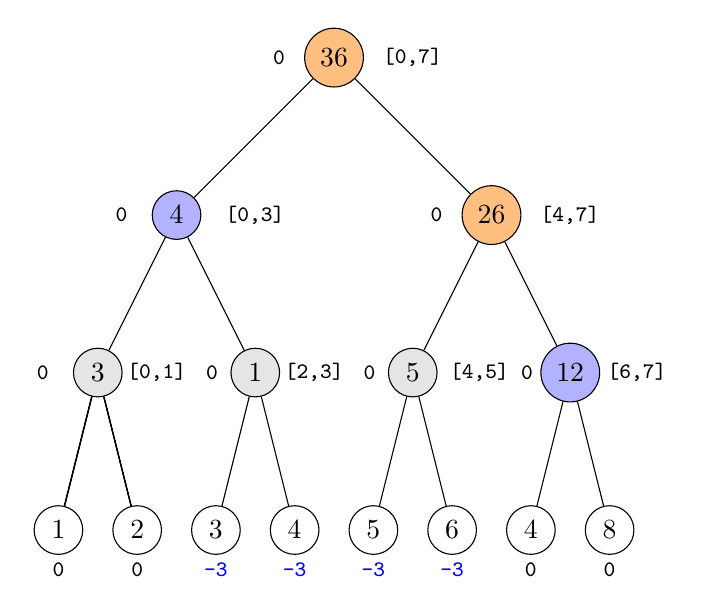
\begin{tikzpicture}
            \node[draw,circle] (A1) at (1, 0) { 1 };
            \node[draw,circle] (A2) at (2, 0) { 2 };
            \node[draw,circle] (A3) at (3, 0) { 3 };
            \node[draw,circle] (A4) at (4, 0) { 4 };
            \node[draw,circle] (A5) at (5, 0) { 5 };
            \node[draw,circle] (A6) at (6, 0) { 6 };
            \node[draw,circle] (A7) at (7, 0) { 4 };
            \node[draw,circle] (A8) at (8, 0) { 8 };

            \node at (1, -.5) { \footnotesize \texttt{\textbf{0}} };
            \node at (2, -.5) { \footnotesize \texttt{\textbf{0}} };
            \node at (3, -.5) { \footnotesize \textcolor{blue}{\texttt{\textbf{-3}}} };
            \node at (4, -.5) { \footnotesize \textcolor{blue}{\texttt{\textbf{-3}}} };
            \node at (5, -.5) { \footnotesize \textcolor{blue}{\texttt{\textbf{-3}}} };
            \node at (6, -.5) { \footnotesize \textcolor{blue}{\texttt{\textbf{-3}}} };
            \node at (7, -.5) { \footnotesize \texttt{\textbf{0}} };
            \node at (8, -.5) { \footnotesize \texttt{\textbf{0}} };
            \node[anchor=east] at (1, 2) { \footnotesize \texttt{\textbf{0}} };
            \node[anchor=east] at (3.15, 2) { \footnotesize \texttt{\textbf{0}} };
            \node[anchor=east] at (5.15, 2) { \footnotesize \texttt{\textbf{0}} };
            \node[anchor=east] at (7.15, 2) { \footnotesize \texttt{\textbf{0}} };
            \node[anchor=east] at (2, 4) { \footnotesize \texttt{\textbf{0}} };
            \node[anchor=east] at (6, 4) { \footnotesize \texttt{\textbf{0}} };
            \node[anchor=east] at (4, 6) { \footnotesize \texttt{\textbf{0}} };
            \node[anchor=west,opacity=0] at (8, 2) { \footnotesize \tt [6,7] };

            \node[draw,circle,fill=gray!20] (B1) at (1.5, 2) { 3 };
            \node[anchor=west] at (1.75, 2) { \footnotesize \tt [0,1] };

            \node[draw,circle,fill=gray!20] (B2) at (3.5, 2) { 1 };
            \node[anchor=west] at (3.75, 2) { \footnotesize \tt [2,3] };

            \node[draw,circle,fill=gray!20] (B3) at (5.5, 2) { 5 };
            \node[anchor=west] at (5.85, 2) { \footnotesize \tt [4,5] };

            \node[draw,circle,fill=blue!30] (B4) at (7.5, 2) { 12 };
            \node[anchor=west] at (7.85, 2) { \footnotesize \tt [6,7] };

            \node[draw,circle,fill=blue!30] (C1) at (2.5, 4) { 4 };
            \node[anchor=west] at (3, 4) { \footnotesize \tt [0,3] };

            \node[draw,circle,fill=orange!50] (C2) at (6.5, 4) { 26 };
            \node[anchor=west] at (7, 4) { \footnotesize \tt [4,7] };

            \node[draw,circle,fill=orange!50] (D1) at (4.5, 6) { 36 };
            \node[anchor=west] at (5, 6) { \footnotesize \tt [0,7] };

            \draw (A1) -- (B1);
            \draw (A2) -- (B1);
            \draw (A3) -- (B2);
            \draw (A4) -- (B2);
            \draw (A5) -- (B3);
            \draw (A6) -- (B3);
            \draw (A7) -- (B4);
            \draw (A8) -- (B4);
            \draw (A1) -- (B1);
            \draw (A2) -- (B1);
            \draw (A1) -- (B1);
            \draw (A2) -- (B1);
            \draw (A1) -- (B1);
            \draw (A2) -- (B1);
            \draw (B1) -- (C1);
            \draw (B2) -- (C1);
            \draw (B3) -- (C2);
            \draw (B4) -- (C2);
            \draw (C1) -- (D1);
            \draw (C2) -- (D1);
        \end{tikzpicture}
    \end{figure}

\end{frame}

\begin{frame}[fragile]{Visualização de update(2, 6, -3)}

    \begin{figure}
        \centering

        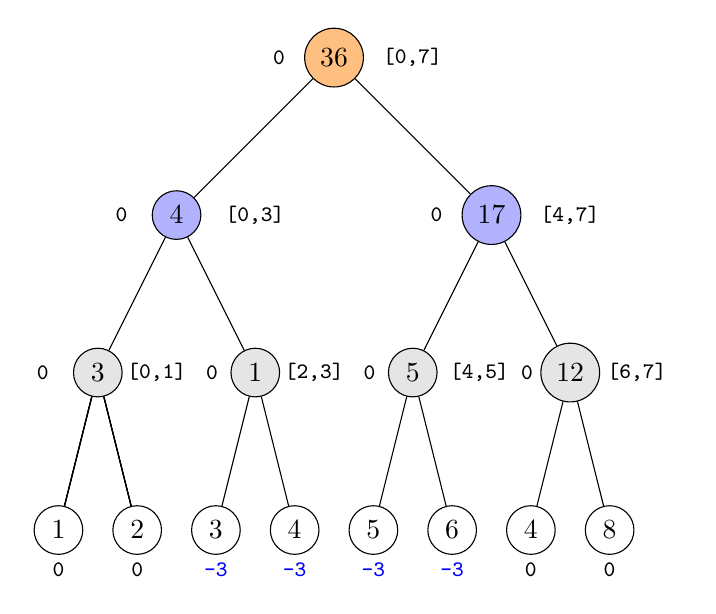
\begin{tikzpicture}
            \node[draw,circle] (A1) at (1, 0) { 1 };
            \node[draw,circle] (A2) at (2, 0) { 2 };
            \node[draw,circle] (A3) at (3, 0) { 3 };
            \node[draw,circle] (A4) at (4, 0) { 4 };
            \node[draw,circle] (A5) at (5, 0) { 5 };
            \node[draw,circle] (A6) at (6, 0) { 6 };
            \node[draw,circle] (A7) at (7, 0) { 4 };
            \node[draw,circle] (A8) at (8, 0) { 8 };

            \node at (1, -.5) { \footnotesize \texttt{\textbf{0}} };
            \node at (2, -.5) { \footnotesize \texttt{\textbf{0}} };
            \node at (3, -.5) { \footnotesize \textcolor{blue}{\texttt{\textbf{-3}}} };
            \node at (4, -.5) { \footnotesize \textcolor{blue}{\texttt{\textbf{-3}}} };
            \node at (5, -.5) { \footnotesize \textcolor{blue}{\texttt{\textbf{-3}}} };
            \node at (6, -.5) { \footnotesize \textcolor{blue}{\texttt{\textbf{-3}}} };
            \node at (7, -.5) { \footnotesize \texttt{\textbf{0}} };
            \node at (8, -.5) { \footnotesize \texttt{\textbf{0}} };
            \node[anchor=east] at (1, 2) { \footnotesize \texttt{\textbf{0}} };
            \node[anchor=east] at (3.15, 2) { \footnotesize \texttt{\textbf{0}} };
            \node[anchor=east] at (5.15, 2) { \footnotesize \texttt{\textbf{0}} };
            \node[anchor=east] at (7.15, 2) { \footnotesize \texttt{\textbf{0}} };
            \node[anchor=east] at (2, 4) { \footnotesize \texttt{\textbf{0}} };
            \node[anchor=east] at (6, 4) { \footnotesize \texttt{\textbf{0}} };
            \node[anchor=east] at (4, 6) { \footnotesize \texttt{\textbf{0}} };
            \node[anchor=west,opacity=0] at (8, 2) { \footnotesize \tt [6,7] };

            \node[draw,circle,fill=gray!20] (B1) at (1.5, 2) { 3 };
            \node[anchor=west] at (1.75, 2) { \footnotesize \tt [0,1] };

            \node[draw,circle,fill=gray!20] (B2) at (3.5, 2) { 1 };
            \node[anchor=west] at (3.75, 2) { \footnotesize \tt [2,3] };

            \node[draw,circle,fill=gray!20] (B3) at (5.5, 2) { 5 };
            \node[anchor=west] at (5.85, 2) { \footnotesize \tt [4,5] };

            \node[draw,circle,fill=gray!20] (B4) at (7.5, 2) { 12 };
            \node[anchor=west] at (7.85, 2) { \footnotesize \tt [6,7] };

            \node[draw,circle,fill=blue!30] (C1) at (2.5, 4) { 4 };
            \node[anchor=west] at (3, 4) { \footnotesize \tt [0,3] };

            \node[draw,circle,fill=blue!30] (C2) at (6.5, 4) { 17 };
            \node[anchor=west] at (7, 4) { \footnotesize \tt [4,7] };

            \node[draw,circle,fill=orange!50] (D1) at (4.5, 6) { 36 };
            \node[anchor=west] at (5, 6) { \footnotesize \tt [0,7] };

            \draw (A1) -- (B1);
            \draw (A2) -- (B1);
            \draw (A3) -- (B2);
            \draw (A4) -- (B2);
            \draw (A5) -- (B3);
            \draw (A6) -- (B3);
            \draw (A7) -- (B4);
            \draw (A8) -- (B4);
            \draw (A1) -- (B1);
            \draw (A2) -- (B1);
            \draw (A1) -- (B1);
            \draw (A2) -- (B1);
            \draw (A1) -- (B1);
            \draw (A2) -- (B1);
            \draw (B1) -- (C1);
            \draw (B2) -- (C1);
            \draw (B3) -- (C2);
            \draw (B4) -- (C2);
            \draw (C1) -- (D1);
            \draw (C2) -- (D1);
        \end{tikzpicture}
    \end{figure}

\end{frame}

\begin{frame}[fragile]{Visualização de update(2, 6, -3)}

    \begin{figure}
        \centering

        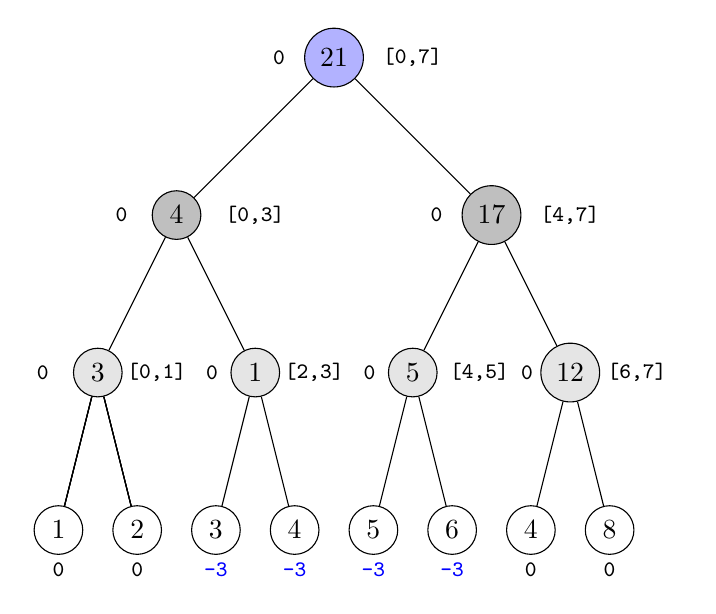
\begin{tikzpicture}
            \node[draw,circle] (A1) at (1, 0) { 1 };
            \node[draw,circle] (A2) at (2, 0) { 2 };
            \node[draw,circle] (A3) at (3, 0) { 3 };
            \node[draw,circle] (A4) at (4, 0) { 4 };
            \node[draw,circle] (A5) at (5, 0) { 5 };
            \node[draw,circle] (A6) at (6, 0) { 6 };
            \node[draw,circle] (A7) at (7, 0) { 4 };
            \node[draw,circle] (A8) at (8, 0) { 8 };

            \node at (1, -.5) { \footnotesize \texttt{\textbf{0}} };
            \node at (2, -.5) { \footnotesize \texttt{\textbf{0}} };
            \node at (3, -.5) { \footnotesize \textcolor{blue}{\texttt{\textbf{-3}}} };
            \node at (4, -.5) { \footnotesize \textcolor{blue}{\texttt{\textbf{-3}}} };
            \node at (5, -.5) { \footnotesize \textcolor{blue}{\texttt{\textbf{-3}}} };
            \node at (6, -.5) { \footnotesize \textcolor{blue}{\texttt{\textbf{-3}}} };
            \node at (7, -.5) { \footnotesize \texttt{\textbf{0}} };
            \node at (8, -.5) { \footnotesize \texttt{\textbf{0}} };
            \node[anchor=east] at (1, 2) { \footnotesize \texttt{\textbf{0}} };
            \node[anchor=east] at (3.15, 2) { \footnotesize \texttt{\textbf{0}} };
            \node[anchor=east] at (5.15, 2) { \footnotesize \texttt{\textbf{0}} };
            \node[anchor=east] at (7.15, 2) { \footnotesize \texttt{\textbf{0}} };
            \node[anchor=east] at (2, 4) { \footnotesize \texttt{\textbf{0}} };
            \node[anchor=east] at (6, 4) { \footnotesize \texttt{\textbf{0}} };
            \node[anchor=east] at (4, 6) { \footnotesize \texttt{\textbf{0}} };
            \node[anchor=west,opacity=0] at (8, 2) { \footnotesize \tt [6,7] };

            \node[draw,circle,fill=gray!20] (B1) at (1.5, 2) { 3 };
            \node[anchor=west] at (1.75, 2) { \footnotesize \tt [0,1] };

            \node[draw,circle,fill=gray!20] (B2) at (3.5, 2) { 1 };
            \node[anchor=west] at (3.75, 2) { \footnotesize \tt [2,3] };

            \node[draw,circle,fill=gray!20] (B3) at (5.5, 2) { 5 };
            \node[anchor=west] at (5.85, 2) { \footnotesize \tt [4,5] };

            \node[draw,circle,fill=gray!20] (B4) at (7.5, 2) { 12 };
            \node[anchor=west] at (7.85, 2) { \footnotesize \tt [6,7] };

            \node[draw,circle,fill=gray!50] (C1) at (2.5, 4) { 4 };
            \node[anchor=west] at (3, 4) { \footnotesize \tt [0,3] };

            \node[draw,circle,fill=gray!50] (C2) at (6.5, 4) { 17 };
            \node[anchor=west] at (7, 4) { \footnotesize \tt [4,7] };

            \node[draw,circle,fill=blue!30] (D1) at (4.5, 6) { 21 };
            \node[anchor=west] at (5, 6) { \footnotesize \tt [0,7] };

            \draw (A1) -- (B1);
            \draw (A2) -- (B1);
            \draw (A3) -- (B2);
            \draw (A4) -- (B2);
            \draw (A5) -- (B3);
            \draw (A6) -- (B3);
            \draw (A7) -- (B4);
            \draw (A8) -- (B4);
            \draw (A1) -- (B1);
            \draw (A2) -- (B1);
            \draw (A1) -- (B1);
            \draw (A2) -- (B1);
            \draw (A1) -- (B1);
            \draw (A2) -- (B1);
            \draw (B1) -- (C1);
            \draw (B2) -- (C1);
            \draw (B3) -- (C2);
            \draw (B4) -- (C2);
            \draw (C1) -- (D1);
            \draw (C2) -- (D1);
        \end{tikzpicture}
    \end{figure}

\end{frame}

\begin{frame}[fragile]{Visualização de update(0, 7, -1)}

    \begin{figure}
        \centering

        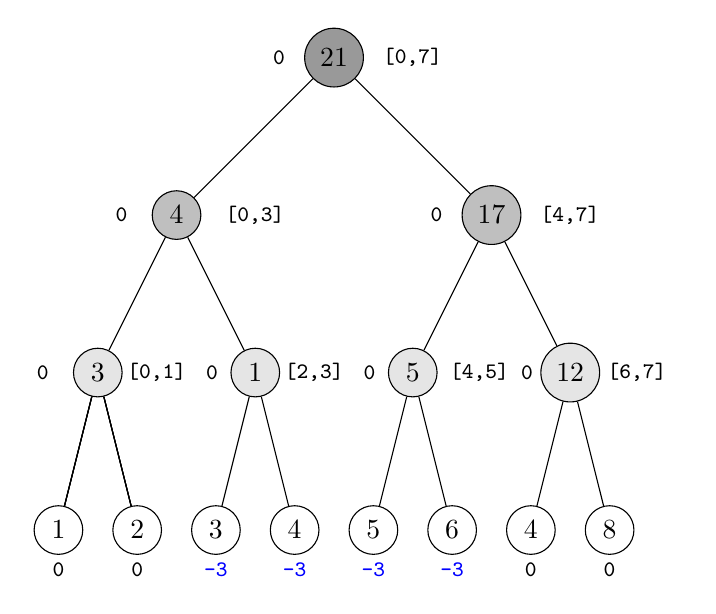
\begin{tikzpicture}
            \node[draw,circle] (A1) at (1, 0) { 1 };
            \node[draw,circle] (A2) at (2, 0) { 2 };
            \node[draw,circle] (A3) at (3, 0) { 3 };
            \node[draw,circle] (A4) at (4, 0) { 4 };
            \node[draw,circle] (A5) at (5, 0) { 5 };
            \node[draw,circle] (A6) at (6, 0) { 6 };
            \node[draw,circle] (A7) at (7, 0) { 4 };
            \node[draw,circle] (A8) at (8, 0) { 8 };

            \node at (1, -.5) { \footnotesize \texttt{\textbf{0}} };
            \node at (2, -.5) { \footnotesize \texttt{\textbf{0}} };
            \node at (3, -.5) { \footnotesize \textcolor{blue}{\texttt{\textbf{-3}}} };
            \node at (4, -.5) { \footnotesize \textcolor{blue}{\texttt{\textbf{-3}}} };
            \node at (5, -.5) { \footnotesize \textcolor{blue}{\texttt{\textbf{-3}}} };
            \node at (6, -.5) { \footnotesize \textcolor{blue}{\texttt{\textbf{-3}}} };
            \node at (7, -.5) { \footnotesize \texttt{\textbf{0}} };
            \node at (8, -.5) { \footnotesize \texttt{\textbf{0}} };
            \node[anchor=east] at (1, 2) { \footnotesize \texttt{\textbf{0}} };
            \node[anchor=east] at (3.15, 2) { \footnotesize \texttt{\textbf{0}} };
            \node[anchor=east] at (5.15, 2) { \footnotesize \texttt{\textbf{0}} };
            \node[anchor=east] at (7.15, 2) { \footnotesize \texttt{\textbf{0}} };
            \node[anchor=east] at (2, 4) { \footnotesize \texttt{\textbf{0}} };
            \node[anchor=east] at (6, 4) { \footnotesize \texttt{\textbf{0}} };
            \node[anchor=east] at (4, 6) { \footnotesize \texttt{\textbf{0}} };
            \node[anchor=west,opacity=0] at (8, 2) { \footnotesize \tt [6,7] };

            \node[draw,circle,fill=gray!20] (B1) at (1.5, 2) { 3 };
            \node[anchor=west] at (1.75, 2) { \footnotesize \tt [0,1] };

            \node[draw,circle,fill=gray!20] (B2) at (3.5, 2) { 1 };
            \node[anchor=west] at (3.75, 2) { \footnotesize \tt [2,3] };

            \node[draw,circle,fill=gray!20] (B3) at (5.5, 2) { 5 };
            \node[anchor=west] at (5.85, 2) { \footnotesize \tt [4,5] };

            \node[draw,circle,fill=gray!20] (B4) at (7.5, 2) { 12 };
            \node[anchor=west] at (7.85, 2) { \footnotesize \tt [6,7] };

            \node[draw,circle,fill=gray!50] (C1) at (2.5, 4) { 4 };
            \node[anchor=west] at (3, 4) { \footnotesize \tt [0,3] };

            \node[draw,circle,fill=gray!50] (C2) at (6.5, 4) { 17 };
            \node[anchor=west] at (7, 4) { \footnotesize \tt [4,7] };

            \node[draw,circle,fill=gray!80] (D1) at (4.5, 6) { 21 };
            \node[anchor=west] at (5, 6) { \footnotesize \tt [0,7] };

            \draw (A1) -- (B1);
            \draw (A2) -- (B1);
            \draw (A3) -- (B2);
            \draw (A4) -- (B2);
            \draw (A5) -- (B3);
            \draw (A6) -- (B3);
            \draw (A7) -- (B4);
            \draw (A8) -- (B4);
            \draw (A1) -- (B1);
            \draw (A2) -- (B1);
            \draw (A1) -- (B1);
            \draw (A2) -- (B1);
            \draw (A1) -- (B1);
            \draw (A2) -- (B1);
            \draw (B1) -- (C1);
            \draw (B2) -- (C1);
            \draw (B3) -- (C2);
            \draw (B4) -- (C2);
            \draw (C1) -- (D1);
            \draw (C2) -- (D1);
        \end{tikzpicture}
    \end{figure}

\end{frame}

\begin{frame}[fragile]{Visualização de update(0, 7, -1)}

    \begin{figure}
        \centering

        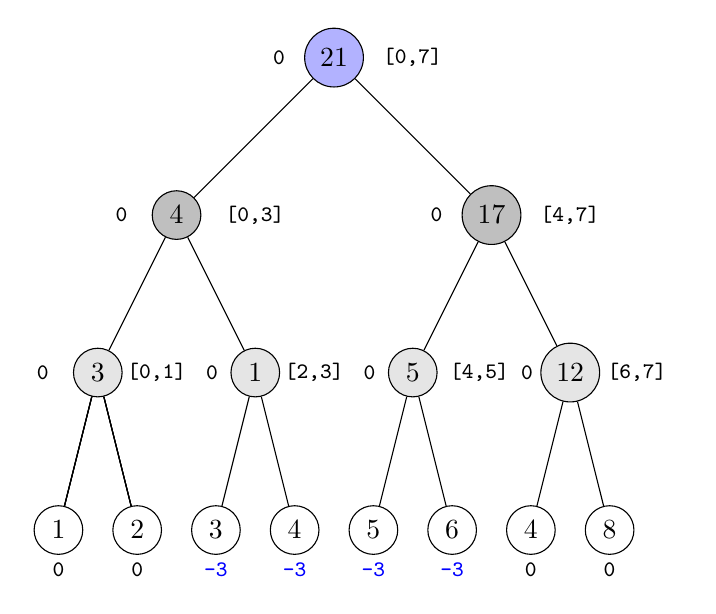
\begin{tikzpicture}
            \node[draw,circle] (A1) at (1, 0) { 1 };
            \node[draw,circle] (A2) at (2, 0) { 2 };
            \node[draw,circle] (A3) at (3, 0) { 3 };
            \node[draw,circle] (A4) at (4, 0) { 4 };
            \node[draw,circle] (A5) at (5, 0) { 5 };
            \node[draw,circle] (A6) at (6, 0) { 6 };
            \node[draw,circle] (A7) at (7, 0) { 4 };
            \node[draw,circle] (A8) at (8, 0) { 8 };

            \node at (1, -.5) { \footnotesize \texttt{\textbf{0}} };
            \node at (2, -.5) { \footnotesize \texttt{\textbf{0}} };
            \node at (3, -.5) { \footnotesize \textcolor{blue}{\texttt{\textbf{-3}}} };
            \node at (4, -.5) { \footnotesize \textcolor{blue}{\texttt{\textbf{-3}}} };
            \node at (5, -.5) { \footnotesize \textcolor{blue}{\texttt{\textbf{-3}}} };
            \node at (6, -.5) { \footnotesize \textcolor{blue}{\texttt{\textbf{-3}}} };
            \node at (7, -.5) { \footnotesize \texttt{\textbf{0}} };
            \node at (8, -.5) { \footnotesize \texttt{\textbf{0}} };
            \node[anchor=east] at (1, 2) { \footnotesize \texttt{\textbf{0}} };
            \node[anchor=east] at (3.15, 2) { \footnotesize \texttt{\textbf{0}} };
            \node[anchor=east] at (5.15, 2) { \footnotesize \texttt{\textbf{0}} };
            \node[anchor=east] at (7.15, 2) { \footnotesize \texttt{\textbf{0}} };
            \node[anchor=east] at (2, 4) { \footnotesize \texttt{\textbf{0}} };
            \node[anchor=east] at (6, 4) { \footnotesize \texttt{\textbf{0}} };
            \node[anchor=east] at (4, 6) { \footnotesize \texttt{\textbf{0}} };
            \node[anchor=west,opacity=0] at (8, 2) { \footnotesize \tt [6,7] };

            \node[draw,circle,fill=gray!20] (B1) at (1.5, 2) { 3 };
            \node[anchor=west] at (1.75, 2) { \footnotesize \tt [0,1] };

            \node[draw,circle,fill=gray!20] (B2) at (3.5, 2) { 1 };
            \node[anchor=west] at (3.75, 2) { \footnotesize \tt [2,3] };

            \node[draw,circle,fill=gray!20] (B3) at (5.5, 2) { 5 };
            \node[anchor=west] at (5.85, 2) { \footnotesize \tt [4,5] };

            \node[draw,circle,fill=gray!20] (B4) at (7.5, 2) { 12 };
            \node[anchor=west] at (7.85, 2) { \footnotesize \tt [6,7] };

            \node[draw,circle,fill=gray!50] (C1) at (2.5, 4) { 4 };
            \node[anchor=west] at (3, 4) { \footnotesize \tt [0,3] };

            \node[draw,circle,fill=gray!50] (C2) at (6.5, 4) { 17 };
            \node[anchor=west] at (7, 4) { \footnotesize \tt [4,7] };

            \node[draw,circle,fill=blue!30] (D1) at (4.5, 6) { 21 };
            \node[anchor=west] at (5, 6) { \footnotesize \tt [0,7] };

            \draw (A1) -- (B1);
            \draw (A2) -- (B1);
            \draw (A3) -- (B2);
            \draw (A4) -- (B2);
            \draw (A5) -- (B3);
            \draw (A6) -- (B3);
            \draw (A7) -- (B4);
            \draw (A8) -- (B4);
            \draw (A1) -- (B1);
            \draw (A2) -- (B1);
            \draw (A1) -- (B1);
            \draw (A2) -- (B1);
            \draw (A1) -- (B1);
            \draw (A2) -- (B1);
            \draw (B1) -- (C1);
            \draw (B2) -- (C1);
            \draw (B3) -- (C2);
            \draw (B4) -- (C2);
            \draw (C1) -- (D1);
            \draw (C2) -- (D1);
        \end{tikzpicture}
    \end{figure}

\end{frame}

\begin{frame}[fragile]{Visualização de update(0, 7, -1)}

    \begin{figure}
        \centering

        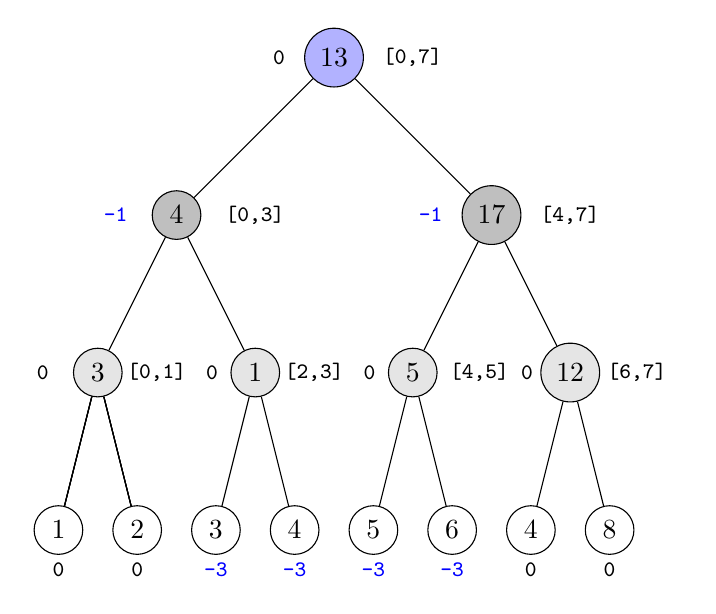
\begin{tikzpicture}
            \node[draw,circle] (A1) at (1, 0) { 1 };
            \node[draw,circle] (A2) at (2, 0) { 2 };
            \node[draw,circle] (A3) at (3, 0) { 3 };
            \node[draw,circle] (A4) at (4, 0) { 4 };
            \node[draw,circle] (A5) at (5, 0) { 5 };
            \node[draw,circle] (A6) at (6, 0) { 6 };
            \node[draw,circle] (A7) at (7, 0) { 4 };
            \node[draw,circle] (A8) at (8, 0) { 8 };

            \node at (1, -.5) { \footnotesize \texttt{\textbf{0}} };
            \node at (2, -.5) { \footnotesize \texttt{\textbf{0}} };
            \node at (3, -.5) { \footnotesize \textcolor{blue}{\texttt{\textbf{-3}}} };
            \node at (4, -.5) { \footnotesize \textcolor{blue}{\texttt{\textbf{-3}}} };
            \node at (5, -.5) { \footnotesize \textcolor{blue}{\texttt{\textbf{-3}}} };
            \node at (6, -.5) { \footnotesize \textcolor{blue}{\texttt{\textbf{-3}}} };
            \node at (7, -.5) { \footnotesize \texttt{\textbf{0}} };
            \node at (8, -.5) { \footnotesize \texttt{\textbf{0}} };
            \node[anchor=east] at (1, 2) { \footnotesize \texttt{\textbf{0}} };
            \node[anchor=east] at (3.15, 2) { \footnotesize \texttt{\textbf{0}} };
            \node[anchor=east] at (5.15, 2) { \footnotesize \texttt{\textbf{0}} };
            \node[anchor=east] at (7.15, 2) { \footnotesize \texttt{\textbf{0}} };
            \node[anchor=east] at (2, 4) { \footnotesize \textcolor{blue}{\texttt{\textbf{-1}}} };
            \node[anchor=east] at (6, 4) { \footnotesize \textcolor{blue}{\texttt{\textbf{-1}}} };
            \node[anchor=east] at (4, 6) { \footnotesize \texttt{\textbf{0}} };
            \node[anchor=west,opacity=0] at (8, 2) { \footnotesize \tt [6,7] };

            \node[draw,circle,fill=gray!20] (B1) at (1.5, 2) { 3 };
            \node[anchor=west] at (1.75, 2) { \footnotesize \tt [0,1] };

            \node[draw,circle,fill=gray!20] (B2) at (3.5, 2) { 1 };
            \node[anchor=west] at (3.75, 2) { \footnotesize \tt [2,3] };

            \node[draw,circle,fill=gray!20] (B3) at (5.5, 2) { 5 };
            \node[anchor=west] at (5.85, 2) { \footnotesize \tt [4,5] };

            \node[draw,circle,fill=gray!20] (B4) at (7.5, 2) { 12 };
            \node[anchor=west] at (7.85, 2) { \footnotesize \tt [6,7] };

            \node[draw,circle,fill=gray!50] (C1) at (2.5, 4) { 4 };
            \node[anchor=west] at (3, 4) { \footnotesize \tt [0,3] };

            \node[draw,circle,fill=gray!50] (C2) at (6.5, 4) { 17 };
            \node[anchor=west] at (7, 4) { \footnotesize \tt [4,7] };

            \node[draw,circle,fill=blue!30] (D1) at (4.5, 6) { 13 };
            \node[anchor=west] at (5, 6) { \footnotesize \tt [0,7] };

            \draw (A1) -- (B1);
            \draw (A2) -- (B1);
            \draw (A3) -- (B2);
            \draw (A4) -- (B2);
            \draw (A5) -- (B3);
            \draw (A6) -- (B3);
            \draw (A7) -- (B4);
            \draw (A8) -- (B4);
            \draw (A1) -- (B1);
            \draw (A2) -- (B1);
            \draw (A1) -- (B1);
            \draw (A2) -- (B1);
            \draw (A1) -- (B1);
            \draw (A2) -- (B1);
            \draw (B1) -- (C1);
            \draw (B2) -- (C1);
            \draw (B3) -- (C2);
            \draw (B4) -- (C2);
            \draw (C1) -- (D1);
            \draw (C2) -- (D1);
        \end{tikzpicture}
    \end{figure}

\end{frame}

\begin{frame}[fragile]{Visualização de update(0, 3, 2)}

    \begin{figure}
        \centering

        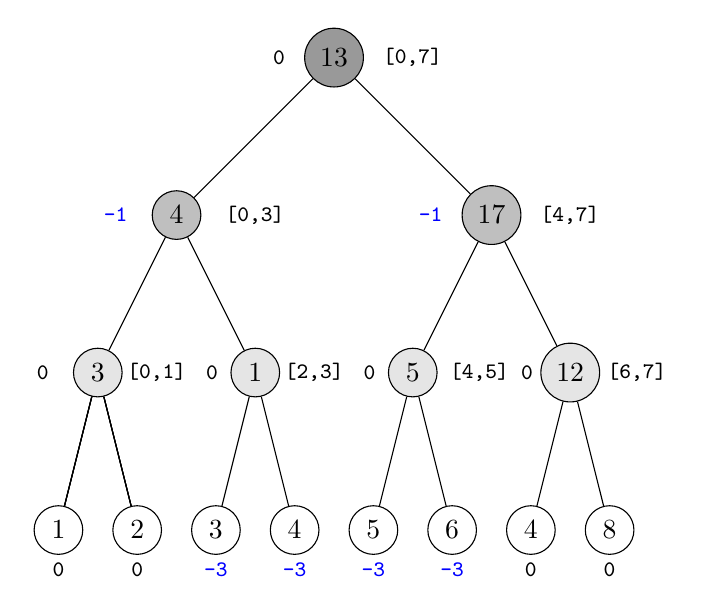
\begin{tikzpicture}
            \node[draw,circle] (A1) at (1, 0) { 1 };
            \node[draw,circle] (A2) at (2, 0) { 2 };
            \node[draw,circle] (A3) at (3, 0) { 3 };
            \node[draw,circle] (A4) at (4, 0) { 4 };
            \node[draw,circle] (A5) at (5, 0) { 5 };
            \node[draw,circle] (A6) at (6, 0) { 6 };
            \node[draw,circle] (A7) at (7, 0) { 4 };
            \node[draw,circle] (A8) at (8, 0) { 8 };

            \node at (1, -.5) { \footnotesize \texttt{\textbf{0}} };
            \node at (2, -.5) { \footnotesize \texttt{\textbf{0}} };
            \node at (3, -.5) { \footnotesize \textcolor{blue}{\texttt{\textbf{-3}}} };
            \node at (4, -.5) { \footnotesize \textcolor{blue}{\texttt{\textbf{-3}}} };
            \node at (5, -.5) { \footnotesize \textcolor{blue}{\texttt{\textbf{-3}}} };
            \node at (6, -.5) { \footnotesize \textcolor{blue}{\texttt{\textbf{-3}}} };
            \node at (7, -.5) { \footnotesize \texttt{\textbf{0}} };
            \node at (8, -.5) { \footnotesize \texttt{\textbf{0}} };
            \node[anchor=east] at (1, 2) { \footnotesize \texttt{\textbf{0}} };
            \node[anchor=east] at (3.15, 2) { \footnotesize \texttt{\textbf{0}} };
            \node[anchor=east] at (5.15, 2) { \footnotesize \texttt{\textbf{0}} };
            \node[anchor=east] at (7.15, 2) { \footnotesize \texttt{\textbf{0}} };
            \node[anchor=east] at (2, 4) { \footnotesize \textcolor{blue}{\texttt{\textbf{-1}}} };
            \node[anchor=east] at (6, 4) { \footnotesize \textcolor{blue}{\texttt{\textbf{-1}}} };
            \node[anchor=east] at (4, 6) { \footnotesize \texttt{\textbf{0}} };
            \node[anchor=west,opacity=0] at (8, 2) { \footnotesize \tt [6,7] };

            \node[draw,circle,fill=gray!20] (B1) at (1.5, 2) { 3 };
            \node[anchor=west] at (1.75, 2) { \footnotesize \tt [0,1] };

            \node[draw,circle,fill=gray!20] (B2) at (3.5, 2) { 1 };
            \node[anchor=west] at (3.75, 2) { \footnotesize \tt [2,3] };

            \node[draw,circle,fill=gray!20] (B3) at (5.5, 2) { 5 };
            \node[anchor=west] at (5.85, 2) { \footnotesize \tt [4,5] };

            \node[draw,circle,fill=gray!20] (B4) at (7.5, 2) { 12 };
            \node[anchor=west] at (7.85, 2) { \footnotesize \tt [6,7] };

            \node[draw,circle,fill=gray!50] (C1) at (2.5, 4) { 4 };
            \node[anchor=west] at (3, 4) { \footnotesize \tt [0,3] };

            \node[draw,circle,fill=gray!50] (C2) at (6.5, 4) { 17 };
            \node[anchor=west] at (7, 4) { \footnotesize \tt [4,7] };

            \node[draw,circle,fill=gray!80] (D1) at (4.5, 6) { 13 };
            \node[anchor=west] at (5, 6) { \footnotesize \tt [0,7] };

            \draw (A1) -- (B1);
            \draw (A2) -- (B1);
            \draw (A3) -- (B2);
            \draw (A4) -- (B2);
            \draw (A5) -- (B3);
            \draw (A6) -- (B3);
            \draw (A7) -- (B4);
            \draw (A8) -- (B4);
            \draw (A1) -- (B1);
            \draw (A2) -- (B1);
            \draw (A1) -- (B1);
            \draw (A2) -- (B1);
            \draw (A1) -- (B1);
            \draw (A2) -- (B1);
            \draw (B1) -- (C1);
            \draw (B2) -- (C1);
            \draw (B3) -- (C2);
            \draw (B4) -- (C2);
            \draw (C1) -- (D1);
            \draw (C2) -- (D1);
        \end{tikzpicture}
    \end{figure}

\end{frame}

\begin{frame}[fragile]{Visualização de update(0, 3, 2)}

    \begin{figure}
        \centering

        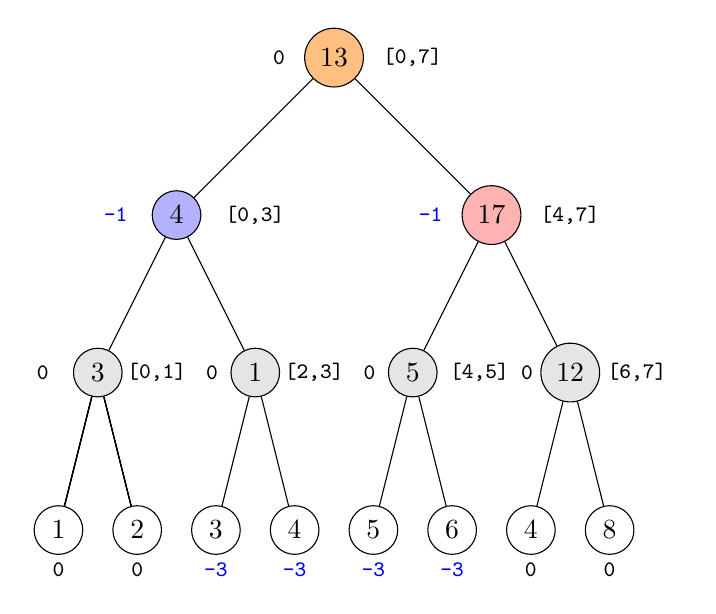
\begin{tikzpicture}
            \node[draw,circle] (A1) at (1, 0) { 1 };
            \node[draw,circle] (A2) at (2, 0) { 2 };
            \node[draw,circle] (A3) at (3, 0) { 3 };
            \node[draw,circle] (A4) at (4, 0) { 4 };
            \node[draw,circle] (A5) at (5, 0) { 5 };
            \node[draw,circle] (A6) at (6, 0) { 6 };
            \node[draw,circle] (A7) at (7, 0) { 4 };
            \node[draw,circle] (A8) at (8, 0) { 8 };

            \node at (1, -.5) { \footnotesize \texttt{\textbf{0}} };
            \node at (2, -.5) { \footnotesize \texttt{\textbf{0}} };
            \node at (3, -.5) { \footnotesize \textcolor{blue}{\texttt{\textbf{-3}}} };
            \node at (4, -.5) { \footnotesize \textcolor{blue}{\texttt{\textbf{-3}}} };
            \node at (5, -.5) { \footnotesize \textcolor{blue}{\texttt{\textbf{-3}}} };
            \node at (6, -.5) { \footnotesize \textcolor{blue}{\texttt{\textbf{-3}}} };
            \node at (7, -.5) { \footnotesize \texttt{\textbf{0}} };
            \node at (8, -.5) { \footnotesize \texttt{\textbf{0}} };
            \node[anchor=east] at (1, 2) { \footnotesize \texttt{\textbf{0}} };
            \node[anchor=east] at (3.15, 2) { \footnotesize \texttt{\textbf{0}} };
            \node[anchor=east] at (5.15, 2) { \footnotesize \texttt{\textbf{0}} };
            \node[anchor=east] at (7.15, 2) { \footnotesize \texttt{\textbf{0}} };
            \node[anchor=east] at (2, 4) { \footnotesize \textcolor{blue}{\texttt{\textbf{-1}}} };
            \node[anchor=east] at (6, 4) { \footnotesize \textcolor{blue}{\texttt{\textbf{-1}}} };
            \node[anchor=east] at (4, 6) { \footnotesize \texttt{\textbf{0}} };
            \node[anchor=west,opacity=0] at (8, 2) { \footnotesize \tt [6,7] };

            \node[draw,circle,fill=gray!20] (B1) at (1.5, 2) { 3 };
            \node[anchor=west] at (1.75, 2) { \footnotesize \tt [0,1] };

            \node[draw,circle,fill=gray!20] (B2) at (3.5, 2) { 1 };
            \node[anchor=west] at (3.75, 2) { \footnotesize \tt [2,3] };

            \node[draw,circle,fill=gray!20] (B3) at (5.5, 2) { 5 };
            \node[anchor=west] at (5.85, 2) { \footnotesize \tt [4,5] };

            \node[draw,circle,fill=gray!20] (B4) at (7.5, 2) { 12 };
            \node[anchor=west] at (7.85, 2) { \footnotesize \tt [6,7] };

            \node[draw,circle,fill=blue!30] (C1) at (2.5, 4) { 4 };
            \node[anchor=west] at (3, 4) { \footnotesize \tt [0,3] };

            \node[draw,circle,fill=red!30] (C2) at (6.5, 4) { 17 };
            \node[anchor=west] at (7, 4) { \footnotesize \tt [4,7] };

            \node[draw,circle,fill=orange!50] (D1) at (4.5, 6) { 13 };
            \node[anchor=west] at (5, 6) { \footnotesize \tt [0,7] };

            \draw (A1) -- (B1);
            \draw (A2) -- (B1);
            \draw (A3) -- (B2);
            \draw (A4) -- (B2);
            \draw (A5) -- (B3);
            \draw (A6) -- (B3);
            \draw (A7) -- (B4);
            \draw (A8) -- (B4);
            \draw (A1) -- (B1);
            \draw (A2) -- (B1);
            \draw (A1) -- (B1);
            \draw (A2) -- (B1);
            \draw (A1) -- (B1);
            \draw (A2) -- (B1);
            \draw (B1) -- (C1);
            \draw (B2) -- (C1);
            \draw (B3) -- (C2);
            \draw (B4) -- (C2);
            \draw (C1) -- (D1);
            \draw (C2) -- (D1);
        \end{tikzpicture}
    \end{figure}

\end{frame}

\begin{frame}[fragile]{Visualização de update(0, 3, 2)}

    \begin{figure}
        \centering

        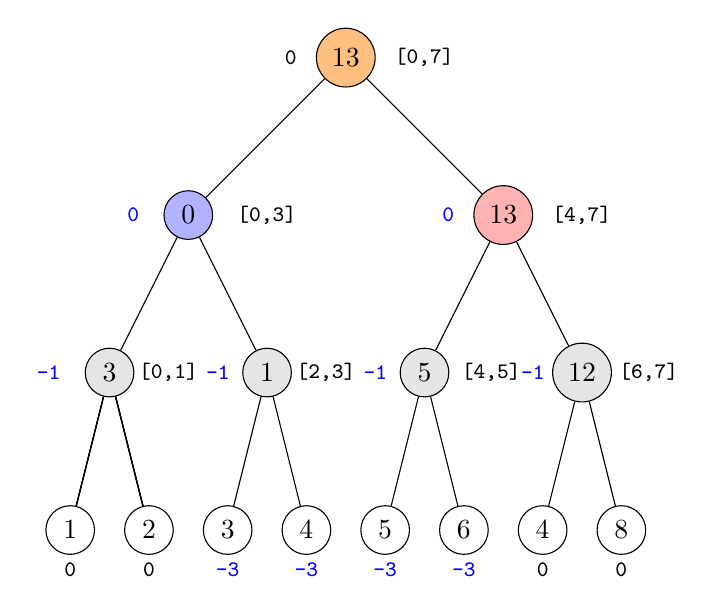
\begin{tikzpicture}
            \node[draw,circle] (A1) at (1, 0) { 1 };
            \node[draw,circle] (A2) at (2, 0) { 2 };
            \node[draw,circle] (A3) at (3, 0) { 3 };
            \node[draw,circle] (A4) at (4, 0) { 4 };
            \node[draw,circle] (A5) at (5, 0) { 5 };
            \node[draw,circle] (A6) at (6, 0) { 6 };
            \node[draw,circle] (A7) at (7, 0) { 4 };
            \node[draw,circle] (A8) at (8, 0) { 8 };

            \node at (1, -.5) { \footnotesize \texttt{\textbf{0}} };
            \node at (2, -.5) { \footnotesize \texttt{\textbf{0}} };
            \node at (3, -.5) { \footnotesize \textcolor{blue}{\texttt{\textbf{-3}}} };
            \node at (4, -.5) { \footnotesize \textcolor{blue}{\texttt{\textbf{-3}}} };
            \node at (5, -.5) { \footnotesize \textcolor{blue}{\texttt{\textbf{-3}}} };
            \node at (6, -.5) { \footnotesize \textcolor{blue}{\texttt{\textbf{-3}}} };
            \node at (7, -.5) { \footnotesize \texttt{\textbf{0}} };
            \node at (8, -.5) { \footnotesize \texttt{\textbf{0}} };
            \node[anchor=east] at (1, 2) { \footnotesize \textcolor{blue}{\texttt{\textbf{-1}}} };
            \node[anchor=east] at (3.15, 2) { \footnotesize \textcolor{blue}{\texttt{\textbf{-1}}} };
            \node[anchor=east] at (5.15, 2) { \footnotesize \textcolor{blue}{\texttt{\textbf{-1}}} };
            \node[anchor=east] at (7.15, 2) { \footnotesize \textcolor{blue}{\texttt{\textbf{-1}}} };
            \node[anchor=east] at (2, 4) { \footnotesize \textcolor{blue}{\texttt{\textbf{0}}} };
            \node[anchor=east] at (6, 4) { \footnotesize \textcolor{blue}{\texttt{\textbf{0}}} };
            \node[anchor=east] at (4, 6) { \footnotesize \texttt{\textbf{0}} };
            \node[anchor=west,opacity=0] at (8, 2) { \footnotesize \tt [6,7] };

            \node[draw,circle,fill=gray!20] (B1) at (1.5, 2) { 3 };
            \node[anchor=west] at (1.75, 2) { \footnotesize \tt [0,1] };

            \node[draw,circle,fill=gray!20] (B2) at (3.5, 2) { 1 };
            \node[anchor=west] at (3.75, 2) { \footnotesize \tt [2,3] };

            \node[draw,circle,fill=gray!20] (B3) at (5.5, 2) { 5 };
            \node[anchor=west] at (5.85, 2) { \footnotesize \tt [4,5] };

            \node[draw,circle,fill=gray!20] (B4) at (7.5, 2) { 12 };
            \node[anchor=west] at (7.85, 2) { \footnotesize \tt [6,7] };

            \node[draw,circle,fill=blue!30] (C1) at (2.5, 4) { 0 };
            \node[anchor=west] at (3, 4) { \footnotesize \tt [0,3] };

            \node[draw,circle,fill=red!30] (C2) at (6.5, 4) { 13 };
            \node[anchor=west] at (7, 4) { \footnotesize \tt [4,7] };

            \node[draw,circle,fill=orange!50] (D1) at (4.5, 6) { 13 };
            \node[anchor=west] at (5, 6) { \footnotesize \tt [0,7] };

            \draw (A1) -- (B1);
            \draw (A2) -- (B1);
            \draw (A3) -- (B2);
            \draw (A4) -- (B2);
            \draw (A5) -- (B3);
            \draw (A6) -- (B3);
            \draw (A7) -- (B4);
            \draw (A8) -- (B4);
            \draw (A1) -- (B1);
            \draw (A2) -- (B1);
            \draw (A1) -- (B1);
            \draw (A2) -- (B1);
            \draw (A1) -- (B1);
            \draw (A2) -- (B1);
            \draw (B1) -- (C1);
            \draw (B2) -- (C1);
            \draw (B3) -- (C2);
            \draw (B4) -- (C2);
            \draw (C1) -- (D1);
            \draw (C2) -- (D1);
        \end{tikzpicture}
    \end{figure}

\end{frame}

\begin{frame}[fragile]{Visualização de update(0, 3, 2)}

    \begin{figure}
        \centering

        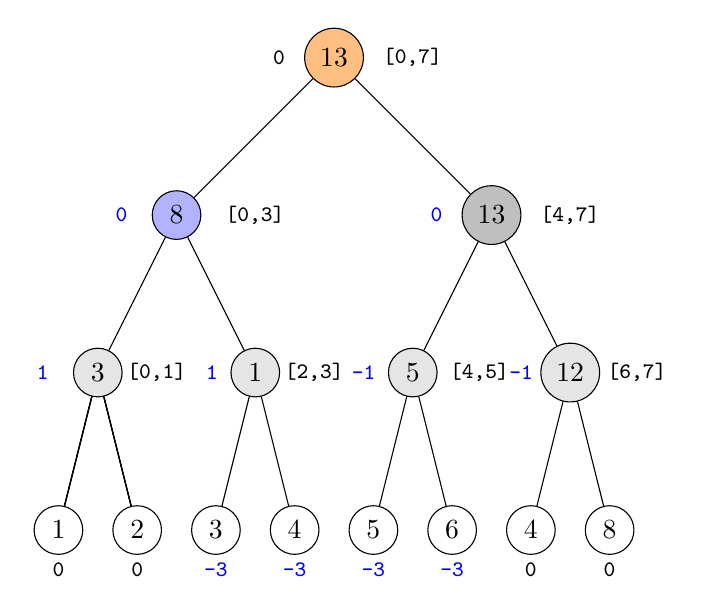
\begin{tikzpicture}
            \node[draw,circle] (A1) at (1, 0) { 1 };
            \node[draw,circle] (A2) at (2, 0) { 2 };
            \node[draw,circle] (A3) at (3, 0) { 3 };
            \node[draw,circle] (A4) at (4, 0) { 4 };
            \node[draw,circle] (A5) at (5, 0) { 5 };
            \node[draw,circle] (A6) at (6, 0) { 6 };
            \node[draw,circle] (A7) at (7, 0) { 4 };
            \node[draw,circle] (A8) at (8, 0) { 8 };

            \node at (1, -.5) { \footnotesize \texttt{\textbf{0}} };
            \node at (2, -.5) { \footnotesize \texttt{\textbf{0}} };
            \node at (3, -.5) { \footnotesize \textcolor{blue}{\texttt{\textbf{-3}}} };
            \node at (4, -.5) { \footnotesize \textcolor{blue}{\texttt{\textbf{-3}}} };
            \node at (5, -.5) { \footnotesize \textcolor{blue}{\texttt{\textbf{-3}}} };
            \node at (6, -.5) { \footnotesize \textcolor{blue}{\texttt{\textbf{-3}}} };
            \node at (7, -.5) { \footnotesize \texttt{\textbf{0}} };
            \node at (8, -.5) { \footnotesize \texttt{\textbf{0}} };
            \node[anchor=east] at (1, 2) { \footnotesize \textcolor{blue}{\texttt{\textbf{1}}} };
            \node[anchor=east] at (3.15, 2) { \footnotesize \textcolor{blue}{\texttt{\textbf{1}}} };
            \node[anchor=east] at (5.15, 2) { \footnotesize \textcolor{blue}{\texttt{\textbf{-1}}} };
            \node[anchor=east] at (7.15, 2) { \footnotesize \textcolor{blue}{\texttt{\textbf{-1}}} };
            \node[anchor=east] at (2, 4) { \footnotesize \textcolor{blue}{\texttt{\textbf{0}}} };
            \node[anchor=east] at (6, 4) { \footnotesize \textcolor{blue}{\texttt{\textbf{0}}} };
            \node[anchor=east] at (4, 6) { \footnotesize \texttt{\textbf{0}} };
            \node[anchor=west,opacity=0] at (8, 2) { \footnotesize \tt [6,7] };

            \node[draw,circle,fill=gray!20] (B1) at (1.5, 2) { 3 };
            \node[anchor=west] at (1.75, 2) { \footnotesize \tt [0,1] };

            \node[draw,circle,fill=gray!20] (B2) at (3.5, 2) { 1 };
            \node[anchor=west] at (3.75, 2) { \footnotesize \tt [2,3] };

            \node[draw,circle,fill=gray!20] (B3) at (5.5, 2) { 5 };
            \node[anchor=west] at (5.85, 2) { \footnotesize \tt [4,5] };

            \node[draw,circle,fill=gray!20] (B4) at (7.5, 2) { 12 };
            \node[anchor=west] at (7.85, 2) { \footnotesize \tt [6,7] };

            \node[draw,circle,fill=blue!30] (C1) at (2.5, 4) { 8 };
            \node[anchor=west] at (3, 4) { \footnotesize \tt [0,3] };

            \node[draw,circle,fill=gray!50] (C2) at (6.5, 4) { 13 };
            \node[anchor=west] at (7, 4) { \footnotesize \tt [4,7] };

            \node[draw,circle,fill=orange!50] (D1) at (4.5, 6) { 13 };
            \node[anchor=west] at (5, 6) { \footnotesize \tt [0,7] };

            \draw (A1) -- (B1);
            \draw (A2) -- (B1);
            \draw (A3) -- (B2);
            \draw (A4) -- (B2);
            \draw (A5) -- (B3);
            \draw (A6) -- (B3);
            \draw (A7) -- (B4);
            \draw (A8) -- (B4);
            \draw (A1) -- (B1);
            \draw (A2) -- (B1);
            \draw (A1) -- (B1);
            \draw (A2) -- (B1);
            \draw (A1) -- (B1);
            \draw (A2) -- (B1);
            \draw (B1) -- (C1);
            \draw (B2) -- (C1);
            \draw (B3) -- (C2);
            \draw (B4) -- (C2);
            \draw (C1) -- (D1);
            \draw (C2) -- (D1);
        \end{tikzpicture}
    \end{figure}

\end{frame}

\begin{frame}[fragile]{Visualização de update(0, 3, 2)}

    \begin{figure}
        \centering

        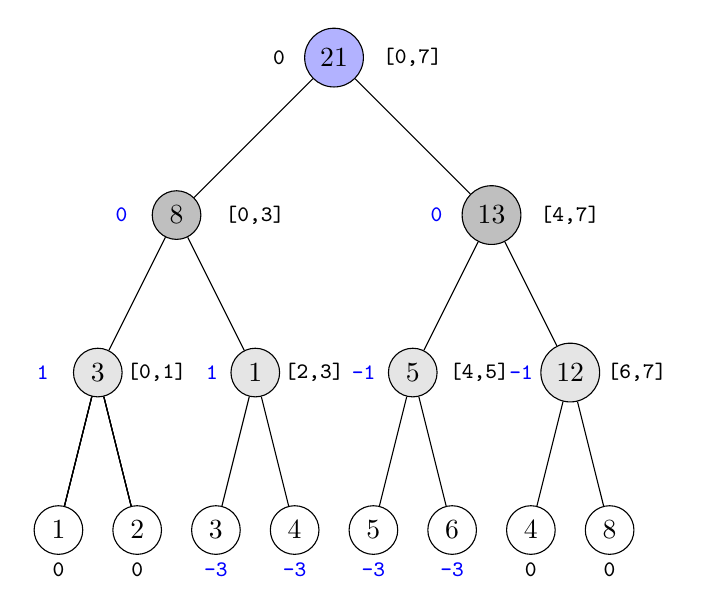
\begin{tikzpicture}
            \node[draw,circle] (A1) at (1, 0) { 1 };
            \node[draw,circle] (A2) at (2, 0) { 2 };
            \node[draw,circle] (A3) at (3, 0) { 3 };
            \node[draw,circle] (A4) at (4, 0) { 4 };
            \node[draw,circle] (A5) at (5, 0) { 5 };
            \node[draw,circle] (A6) at (6, 0) { 6 };
            \node[draw,circle] (A7) at (7, 0) { 4 };
            \node[draw,circle] (A8) at (8, 0) { 8 };

            \node at (1, -.5) { \footnotesize \texttt{\textbf{0}} };
            \node at (2, -.5) { \footnotesize \texttt{\textbf{0}} };
            \node at (3, -.5) { \footnotesize \textcolor{blue}{\texttt{\textbf{-3}}} };
            \node at (4, -.5) { \footnotesize \textcolor{blue}{\texttt{\textbf{-3}}} };
            \node at (5, -.5) { \footnotesize \textcolor{blue}{\texttt{\textbf{-3}}} };
            \node at (6, -.5) { \footnotesize \textcolor{blue}{\texttt{\textbf{-3}}} };
            \node at (7, -.5) { \footnotesize \texttt{\textbf{0}} };
            \node at (8, -.5) { \footnotesize \texttt{\textbf{0}} };
            \node[anchor=east] at (1, 2) { \footnotesize \textcolor{blue}{\texttt{\textbf{1}}} };
            \node[anchor=east] at (3.15, 2) { \footnotesize \textcolor{blue}{\texttt{\textbf{1}}} };
            \node[anchor=east] at (5.15, 2) { \footnotesize \textcolor{blue}{\texttt{\textbf{-1}}} };
            \node[anchor=east] at (7.15, 2) { \footnotesize \textcolor{blue}{\texttt{\textbf{-1}}} };
            \node[anchor=east] at (2, 4) { \footnotesize \textcolor{blue}{\texttt{\textbf{0}}} };
            \node[anchor=east] at (6, 4) { \footnotesize \textcolor{blue}{\texttt{\textbf{0}}} };
            \node[anchor=east] at (4, 6) { \footnotesize \texttt{\textbf{0}} };
            \node[anchor=west,opacity=0] at (8, 2) { \footnotesize \tt [6,7] };

            \node[draw,circle,fill=gray!20] (B1) at (1.5, 2) { 3 };
            \node[anchor=west] at (1.75, 2) { \footnotesize \tt [0,1] };

            \node[draw,circle,fill=gray!20] (B2) at (3.5, 2) { 1 };
            \node[anchor=west] at (3.75, 2) { \footnotesize \tt [2,3] };

            \node[draw,circle,fill=gray!20] (B3) at (5.5, 2) { 5 };
            \node[anchor=west] at (5.85, 2) { \footnotesize \tt [4,5] };

            \node[draw,circle,fill=gray!20] (B4) at (7.5, 2) { 12 };
            \node[anchor=west] at (7.85, 2) { \footnotesize \tt [6,7] };

            \node[draw,circle,fill=gray!50] (C1) at (2.5, 4) { 8 };
            \node[anchor=west] at (3, 4) { \footnotesize \tt [0,3] };

            \node[draw,circle,fill=gray!50] (C2) at (6.5, 4) { 13 };
            \node[anchor=west] at (7, 4) { \footnotesize \tt [4,7] };

            \node[draw,circle,fill=blue!30] (D1) at (4.5, 6) { 21 };
            \node[anchor=west] at (5, 6) { \footnotesize \tt [0,7] };

            \draw (A1) -- (B1);
            \draw (A2) -- (B1);
            \draw (A3) -- (B2);
            \draw (A4) -- (B2);
            \draw (A5) -- (B3);
            \draw (A6) -- (B3);
            \draw (A7) -- (B4);
            \draw (A8) -- (B4);
            \draw (A1) -- (B1);
            \draw (A2) -- (B1);
            \draw (A1) -- (B1);
            \draw (A2) -- (B1);
            \draw (A1) -- (B1);
            \draw (A2) -- (B1);
            \draw (B1) -- (C1);
            \draw (B2) -- (C1);
            \draw (B3) -- (C2);
            \draw (B4) -- (C2);
            \draw (C1) -- (D1);
            \draw (C2) -- (D1);
        \end{tikzpicture}
    \end{figure}

\end{frame}
